\documentclass[14pt, a4paper]{article}
\usepackage[russian]{babel}
\usepackage{graphicx}
\usepackage{tabularx}
% \usepackage{caption}

\title{Windows}

\begin{document}

\begin{center}
\section*{История Windows}
\end{center}

\begin{figure}[h]%current location
    \centering
    \scalebox{0.7}{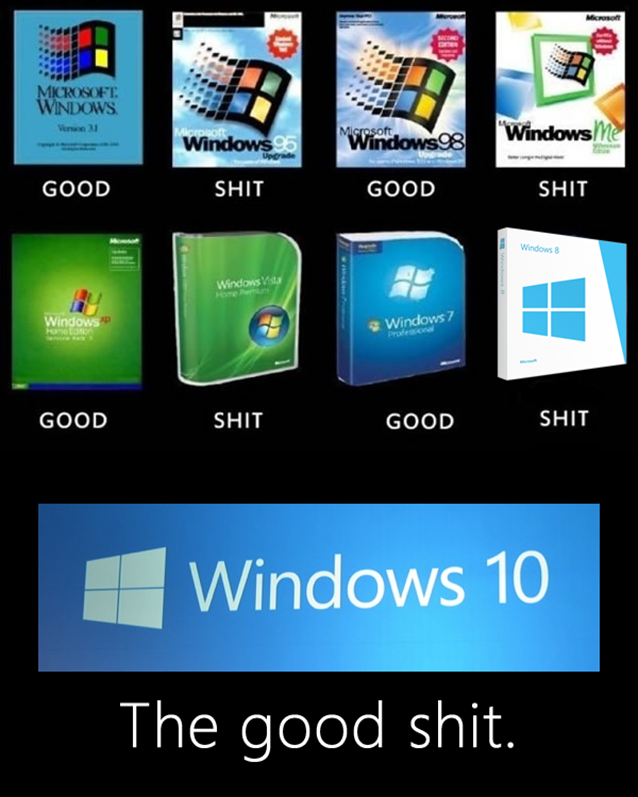
\includegraphics[width=1\textwidth]{imgs/1.1.png}}
    \label{framework} %framework,fig1
\end{figure}

История развития версий \textbf{Windows} – вне сомнения, любопытная тема, которая заслуживает отдельной книги. 
Поэтому мы не будем тщательно переворачивать пыльные фолианты истории и лишь вкратце ознакомимся с ключевыми событиями из жизни \textbf{Microsoft Windows}.


Вопреки расхожему мнению, первая версия \textbf{Windows} вовсе не была самостоятельной операционной системой.
В действительности \textbf{Windows} представляла собой графическую «надстройку» над операционной системой \textbf{DOS} и была призвана упростить работу с темной и мрачной командной строкой. 
Многие пользователи \textbf{DOS} не поняли этого нововведения.


До сих пор в Интернете «гуляет» знаменитый отрывок из книги советских инженеров,
выпущенной в 1989 году. Книга называется «\textbf{Персональные ЭВМ в инженерной практике}»,
и суровые инженеры следующим образом отозвались о продукте \textbf{Microsoft}.


«Одним из примеров громоздкой и, по мнению авторов, бесполезной надстройки является интегрированная система \textbf{WINDOWS} фирмы \textbf{Microsoft}.
Эта система занимает почти 1 Мбайт дисковой памяти и рассчитана на преимущественное использование совместно с устройством типа «мышь»…
Таким образом, читатель уже понял, что среди надстроек над ДОС бывают довольно бесполезные системы, которые только выглядят красиво,
а на самом деле отнимают время пользователя, память на дисках и оперативную память ЭВМ. Обманчивая красота таких систем, однако, сильно воздействует на неискушенных пользователей,
которые не имели практики работы на машине. Инерция мышления бывает столь сильна, что авторам приходилось наблюдать, как люди, начавшие работать с подобной настройкой,
впоследствии с трудом заставляют себя изучать команды ДОС. Хочется предостеречь от этой ошибки читателя».


В начале 80-х годов прошлого века компания \textbf{IBM} работала над персональным компьютером на базе процессора \textbf{Intel 8088}.
С середины 70 годов компания \textbf{Microsoft} была основным поставщиком \textbf{Basic} для восьмибитных микрокомпьютеров.
Когда \textbf{IBM} обратилась к \textbf{Microsoft} для лицензирования \textbf{Basic} для их нового компьютера \textbf{IBM PC}, \textbf{Microsoft} согласилась,
а также посоветовала обратиться к компании \textbf{Digital Research} для лицензирования операционной системы \textbf{\underline{CP/M}}.
Но, получилось так, что глава \textbf{Digital Research} не нашел в своем графике времени для встречи для \textbf{IBM},
и \textbf{IBM} снова обратилась к \textbf{Microsoft}, теперь уже с просьбой решить вопрос операционной системы для \textbf{IBM PC}.
\textbf{Microsoft} купила клон \textbf{ОС CP/M} у компании \textbf{Seattle Computer Products} и перенесла её на \textbf{IBM PC}.
Итоговым названием получившейся ОС стало \textbf{\underline{MS-DOS 1.0}}.

\begin{figure}[h]%current location
    \centering
    \scalebox{1}{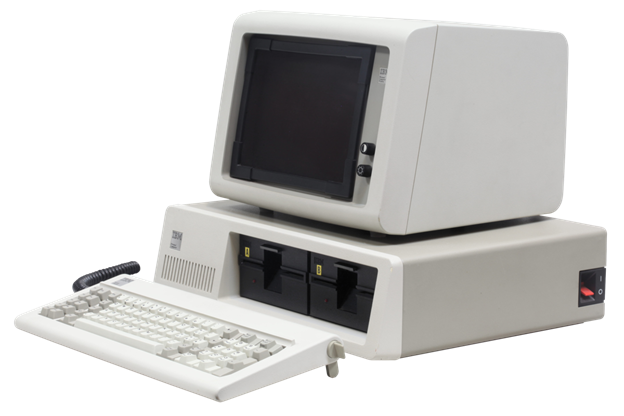
\includegraphics[width=1\textwidth]{imgs/1.2.png}}
    \textit{\caption{IBM PC}}
    \label{framework} %framework,fig1
\end{figure}


Первые продукты с названием «\textbf{Windows}» от \textbf{Microsoft} не были операционными системами. Это были графические среды для \textbf{MS-DOS}.
На фоне успеха, в том числе и коммерческого, пользовательского интерфейса на \textbf{\underline{Apple Lisa}},
компания решила реализовать графический интерфейс на \textbf{IBM PC} с \textbf{MS-DOS}. В отличии от относительно дешевых \textbf{IBM PC}, \textbf{Apple Lisa} стоили дорого (почти 10 тысяч долларов),
и немногие покупатели могли позволить купить их. \textbf{Microsoft} решила занять нишу дешевых компьютеров с графическим интерфейсом.
При этом низкая стоимость достигалась экономией на комплектующих и более низкая производительность, по сравнению с \textbf{Lisa},
избежать не получилось. Так, в 1985, 1987 и в 1990 выходят первые три версии \textbf{Windows} — 1.0, 2.0 и 3.0.
Причем за первые шесть месяцев после релиза \textbf{Windows} 3.0 было продано более 1 миллиона экземпляров.
Дальнейшее развитие \textbf{Windows} можно разделить на два направления — \textbf{Windows} на базе \textbf{MS-DOS} и \textbf{Windows} на базе \textbf{NT}.


\begin{figure}[h]%current location
    \centering
    \scalebox{1}{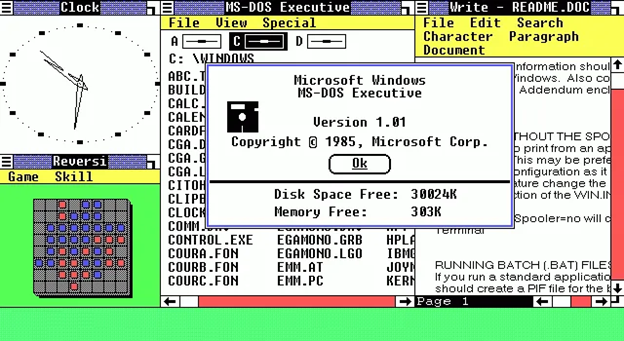
\includegraphics[width=1\textwidth]{imgs/1.3.png}}
    \textit{\caption{Windows 1.01}}
    \label{framework} %framework,fig1
\end{figure}


\begin{center}
    \subsection*{Windows 1.0 — 20 нoябpя 1985 гoдa}
\end{center}


Компания \textbf{Microsoft} - 20 ноября 1985 официально выпустила \textbf{Windows 1.0}
(программная оболочка для \textbf{MS-DOS}).
Системные требования: наличие жесткого диска или двух дискет, 256 КБ оперативной памяти,
графический адаптер, \textbf{MS-DOS 2.0}.
Операционная система \textbf{Windows 1.0} не набрала такой популярности как \textbf{Macintosh} от \textbf{Apple}.
В итоге \textbf{Microsoft} поддерживала \textbf{Windows 1.0} целых 16 лет, до 31 декабря 2001 года.\newpage


\begin{centering}
    \subsection*{Windows 2.0 — 9 декабря 1987}
\end{centering}

Вторая версия \textbf{Windows} выходит с улучшенной графикой. Новые процессоры intel 286 и
intel 386 позволили расширить возможности \textbf{Windows 2.0}.
На рабочем столе появились значки, возможность запуск нескольких окон, которые можно наложить друг на друга,
теперь пользователь может взаимодействовать с системой используя «горячие» комбинации клавиш.
\textbf{Windows 2.0} сделала компанию \textbf{Microsoft} – самой крупной в разработке программного обеспечения.

\begin{figure}[h]%current location
    \centering
    \scalebox{1}{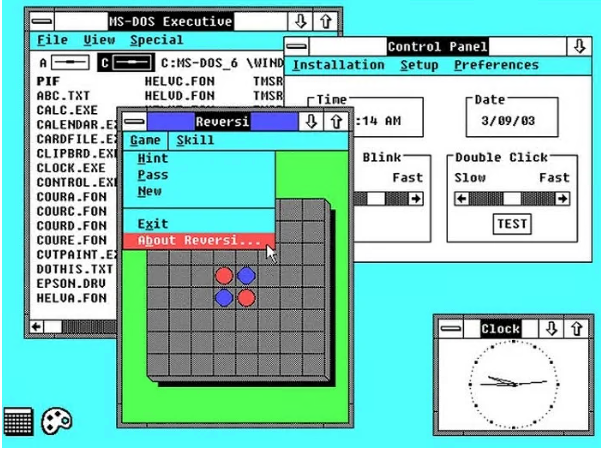
\includegraphics[width=1\textwidth]{imgs/3.1.png}}
    \label{framework} %framework,fig1
\end{figure}\newpage


\begin{centering}
    \subsection*{Windows 3.0 — 22 мая 1990 года}
\end{centering}

\begin{figure}[h]%current location
    \centering
    \scalebox{1}{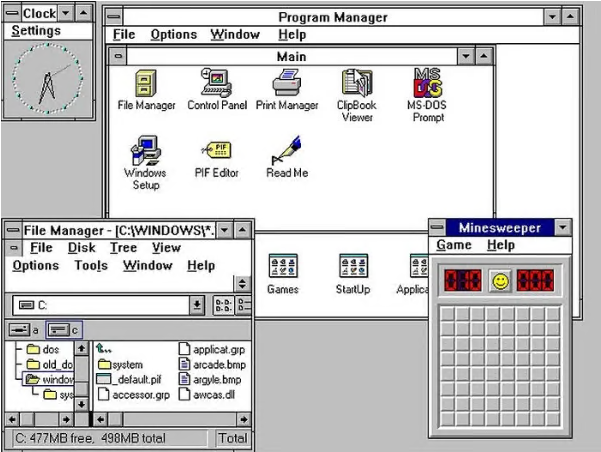
\includegraphics[width=1\textwidth]{imgs/4.1.png}}
    \label{framework} %framework,fig1
\end{figure}

С версии \textbf{Windows 3.0} – начинается успех системы. Новый пользовательский интерфейс (16-цветовых гамм).
Под \textbf{Windows 3.0} выходит пакет офисных приложений \textbf{Microsoft Office}, который включал
\textbf{Word}, \textbf{Excel} и \textbf{Powerpoint}.
За 2 года было продано 10 миллионов лицензий.
Игра «Сапер» — сыграла большую роль в успехе \textbf{Windows 3.0},
игра и сейчас помогает офисным менеджерам скоротать время на работе.\newpage

\begin{centering}
    \subsection*{Windows NT 3.1 — 27 июля 1993 года}
\end{centering}

\begin{figure}[h]%current location
    \centering
    \scalebox{1}{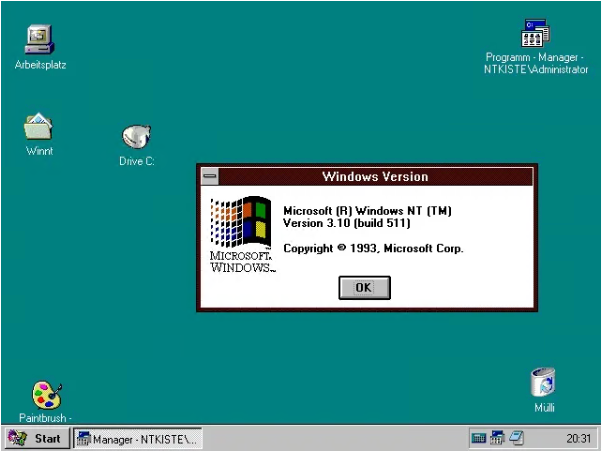
\includegraphics[width=1\textwidth]{imgs/5.1.png}}
    \label{framework} %framework,fig1
\end{figure}

Следующая 32-битная система \textbf{Windows NT 3.1} была нацелена на корпоративных клиентов,
включала интегрированные сети, многозадачный планировщик Windows,
поддержку нескольких процессорных архитектур. Тогда впервые появилась файловая система \textbf{NTFS}.
Среди опытных пользователей \textbf{Windows NT 3.1} называли самой стабильной операционной системой.\newpage

\begin{centering}
    \subsection*{Windows 9x}
\end{centering}

Windows на базе \textbf{MS-DOS} или \textbf{Windows 9x} не были первыми ОС от \textbf{Microsoft},
но они продолжали «старые традиции» и были построены на основе 16-битного кода \textbf{MS-DOS}.
В августе 1995 года была выпущена \textbf{Windows 95} — первая система семейства \textbf{Windows 9x}. Она уже была полноценной
операционной системой с соответствующими возможностями. Однако у системы были проблемы с безопасностью
(например, не было «администратора») и с изоляцией приложений. Зависание 16-битного приложения приводило к блокировке всей системы.
Проблемы со стабильностью достались и \textbf{Windows 98} и \textbf{Windows ME},
которые отличались от выпуска 95 года рядом небольших обновлений. 

\begin{figure}[h]%current location
    \centering
    \scalebox{1}{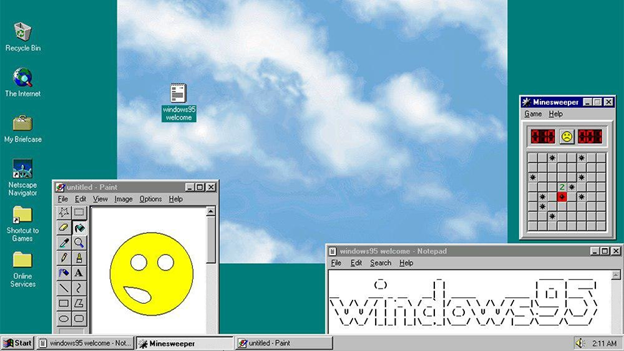
\includegraphics[width=1\textwidth]{imgs/6.1.png}}
    \textit{\caption{Windows 95}}
    \label{framework} %framework,fig1
\end{figure} \newpage


\begin{centering}
    \subsection*{Windows NT}
\end{centering}

В целом, к концу 80-х годов в \textbf{Microsoft} появилось понимание о необходимости
разработки операционной системы не на базе \textbf{MS-DOS}.
Параллельно с разработкой софта, связанного с MS-DOS, \textbf{Microsoft}
наняла команду инженеров из компании \textbf{DEC} для разработки новой
32-битной операционной системы. Главой группы стал Дэйв Катлер — один из главных разработчиков \textbf{ОС VMS}.
Новая система была названа \textbf{NT} — от сокращения \textbf{New Technology}.
Основной упор при разработке \textbf{NT} делался на безопасность и надежность системы,
а также на совместимость с \textbf{Windows} на \textbf{MS-DOS}.
Так получилось, что опыт при разработке \textbf{VMS} повлиял на \textbf{NT} и сходство между ними стало
причиной спора между \textbf{DEC} и \textbf{Microsoft}. По итогу спор был решен во внесудебном порядке. 

\begin{figure}[h]%current location
    \centering
    \scalebox{1}{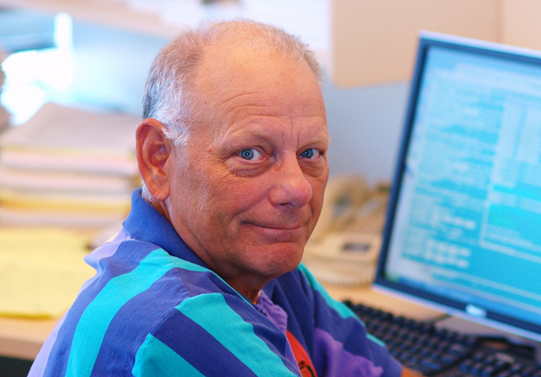
\includegraphics[width=1\textwidth]{imgs/7.1.png}}
    \textit{\caption{Дэйв Катлер}}
    \label{framework} %framework,fig1
\end{figure}

Первая система \textbf{Windows} называлась \textbf{Windows NT 3.1} и была выпущена в 1993 году.
Это была первая ОС от \textbf{Microsoft}. Индекс 3.1 был выбран для соответствия \textbf{Windows 3.1} на \textbf{MS-DOS}.
Эта версия не имела особого успеха. Для \textbf{NT} требовалось больше памяти,
32-разрядных приложений на рынке было мало, возникали проблемы с совместимостью драйвером. Достичь поставленных целей смогли в NT 3.5.
А первым серьезным обновлением для \textbf{NT} стала версия 4.0 в 96 году. Теперь эта система была мощна, надежна и безопасна,
а также обеспечивала тот же интерфейс, что и \textbf{Windows 95} (которая к тому моменту была чрезвычайно популярной). 

\begin{figure}[h]%current location
    \centering
    \scalebox{0.7}{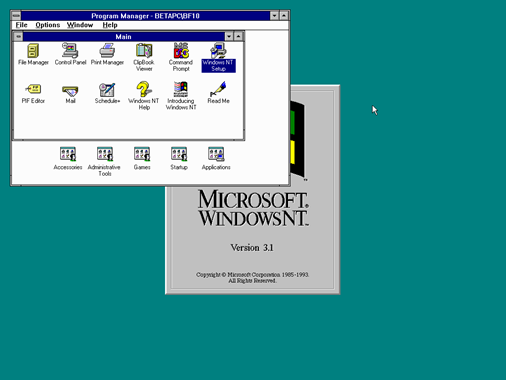
\includegraphics[width=1\textwidth]{imgs/7.2.png}}
    \textit{\caption{Windows NT 3.1}}
    \label{framework} %framework,fig1
\end{figure}


% ??????????????????????????????????
В 2000 году вышла новая версия \textbf{Windows} — \textbf{Windows 2000}. Она развивала идеи, заложенные в системы NT.
Был добавлена технология \textbf{Plug-and-Play}, управление электропитанием и улучшен интерфейс пользователя. 


Домашняя операционная система не получилась. \textbf{Windows 2000 Professional} вышла для бизнеса рынка (корпоративная система),
в которой реализовали простую установку оборудования, беспроводные устройства, поддержку USB-устройств, инфракрасные устройства и
IEEE 1394, a также массу уязвимостей, которые следующие 10 лет лечили c помощью множества обновлений.
Пользователи поверили рекламе \textbf{Microsoft}, которая показывала,
что \textbf{Windows 2000} самая безопасная операционная система,
так как она принадлежала к семейству \textbf{Windows NT}. Пользователи c большим
рвением устанавливали \textbf{Windows 2000} на домашний компьютер.


\begin{figure}[h]%current location
    \centering
    \scalebox{0.7}{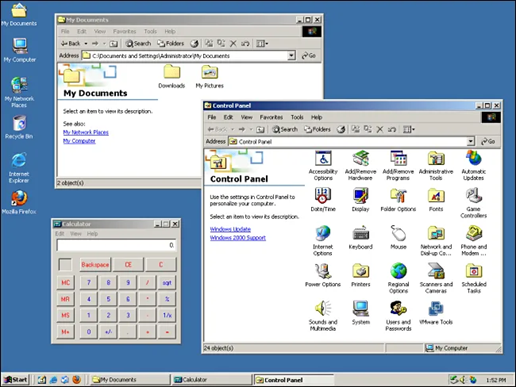
\includegraphics[width=1\textwidth]{imgs/7.3.png}}
    \textit{\caption{Windows 2000}}
    \label{framework} %framework,fig1
\end{figure} \newpage


\begin{centering}
    \subsection*{Windows XP — 25 октября 2001 года}
\end{centering}

Успех \textbf{Windows 2000} задал вектор развития для следующего поколения — \textbf{Windows XP}.
В «хрюшке» \textbf{Microsoft} улучшила совместимость, интерфейс стал более дружелюбным.
Стратегия \textbf{Microsoft} завоевывать аудиторию уже знакомыми системами дала плоды — за несколько лет
\textbf{Windows XP} была установлена на сотнях миллионах ПК. Эпоха \textbf{MS-DOS} подошла к концу.

\begin{figure}[h]%current location
    \centering
    \scalebox{1}{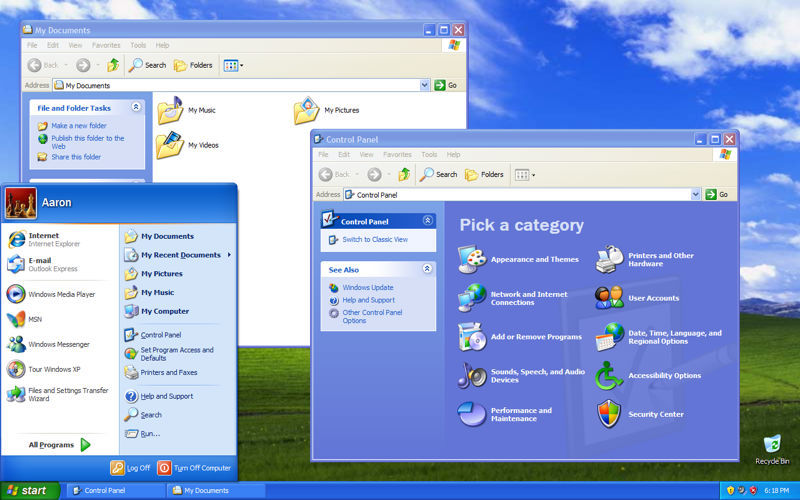
\includegraphics[width=1\textwidth]{imgs/8.1.png}}
    \textit{\caption{Windows XP}}
    \label{framework} %framework,fig1
\end{figure} \newpage


\begin{centering}
    \subsection*{Windows Vista — 30 января 2007 года}
\end{centering}


Следующий проект \textbf{Microsoft} пал жертвой собственных амбиций. Через пять лет после \textbf{Windows XP},
в 2006 году на свет вышла \textbf{Windows Vista}. В ней был переделан графический интерфейс, переработаны и добавлены
функциональные возможности в плане безопасности. Была улучшена производительность, надежность.


Первоначальные планы \textbf{Microsoft} по поводу \textbf{Vista} были настолько обширны, что через несколько лет после
начала разработки проект пришлось сильно ограничить. \textbf{Vista} включала в себе 70 миллионов строк кода,
часть которого составлял «причесанный» код \textbf{XP}. Неудача \textbf{Vista} отчасти с тем, что она вышла не в то время.
На 2006 год пришелся бум недорогих компьютеров, которые не могли обеспечить достаточную для \textbf{Vista} производительность.

\begin{figure}[h]%current location
    \centering
    \scalebox{1}{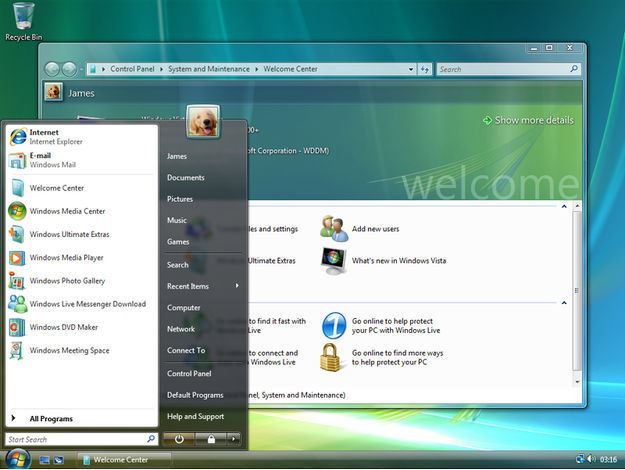
\includegraphics[width=1\textwidth]{imgs/9.1.png}}
    \textit{\caption{Windows Vista}}
    \label{framework} %framework,fig1
\end{figure} \newpage


\begin{centering}
    \subsection*{Windows 7 — 22 октября 2009 года}
\end{centering}

Проблемы \textbf{Vista} были учтены при разработке Windows 7. \textbf{Microsoft} уделила большее внимание тестированию
и производительности новой системы. \textbf{Windows 7} быстро вытеснила \textbf{Vista}, а затем и \textbf{XP},
став самой популярной версией \textbf{Windows} до появления \textbf{Windows 10}
(сейчас \textbf{Windows 7} на втором месте по популярности).

\begin{figure}[h]%current location
    \centering
    \scalebox{1}{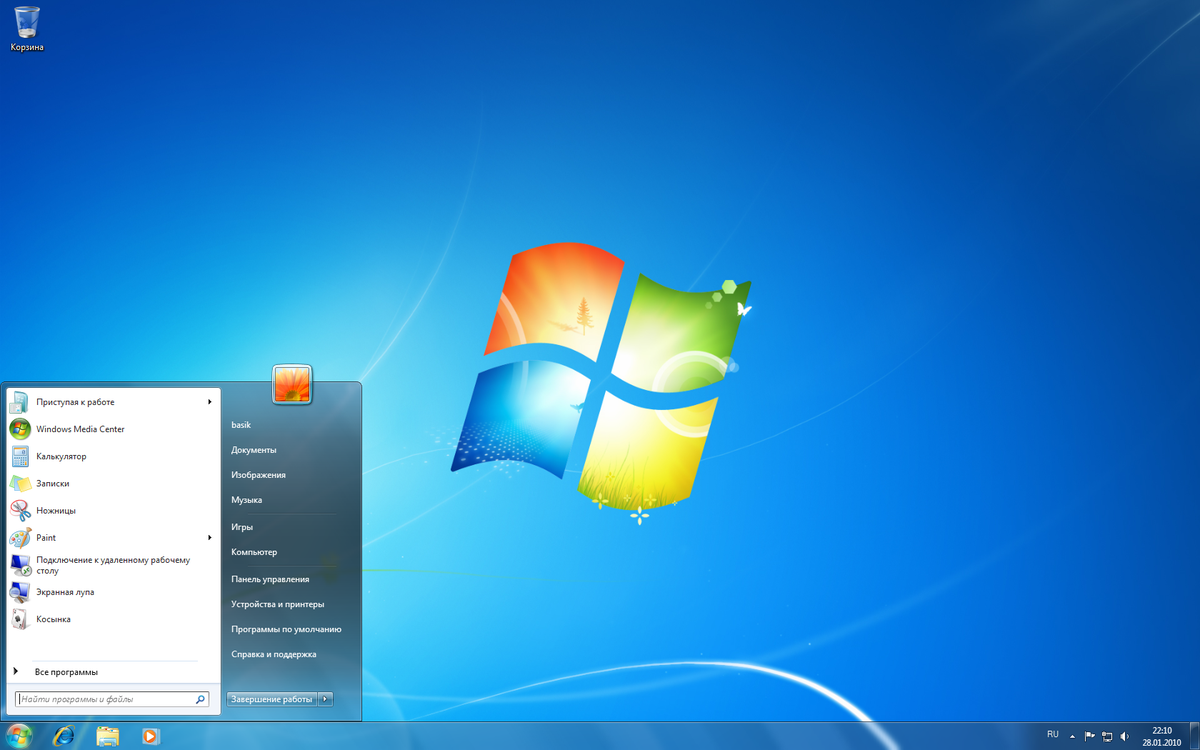
\includegraphics[width=1\textwidth]{imgs/10.1.png}}
    \textit{\caption{Windows 7}}
    \label{framework} %framework,fig1
\end{figure} \newpage

\begin{centering}
    \subsection*{Windows 8 — 26 октября 2012 года}
\end{centering}

Бум смартфонов в начале 2010-х подтолкнул \textbf{Microsoft} к созданию операционной системы, которую можно было
бы развернуть на разных устройствах: на телефонах, планшетах, приставках и т. д. В результате этой
работы мир узрел \textbf{Windows 8}. «Восьмерка» построена на модульном подходе MinWin для получения небольшого ядра \textbf{ОС},
которое можно было бы расширить на линейку других типов устройств. Но аудитория встретила холодно такой подход.
Многие люди критиковали «смартфоноподобный» интерфейс на ПК, отсутствие кнопки пуск.
Для решения многих проблем \textbf{Microsoft} выпустила обновление под названием \textbf{Windows 8.1}, которая,
помимо исправления имеющихся ошибок, добавила новые функции. 

\begin{figure}[h]%current location
    \centering
    \scalebox{1}{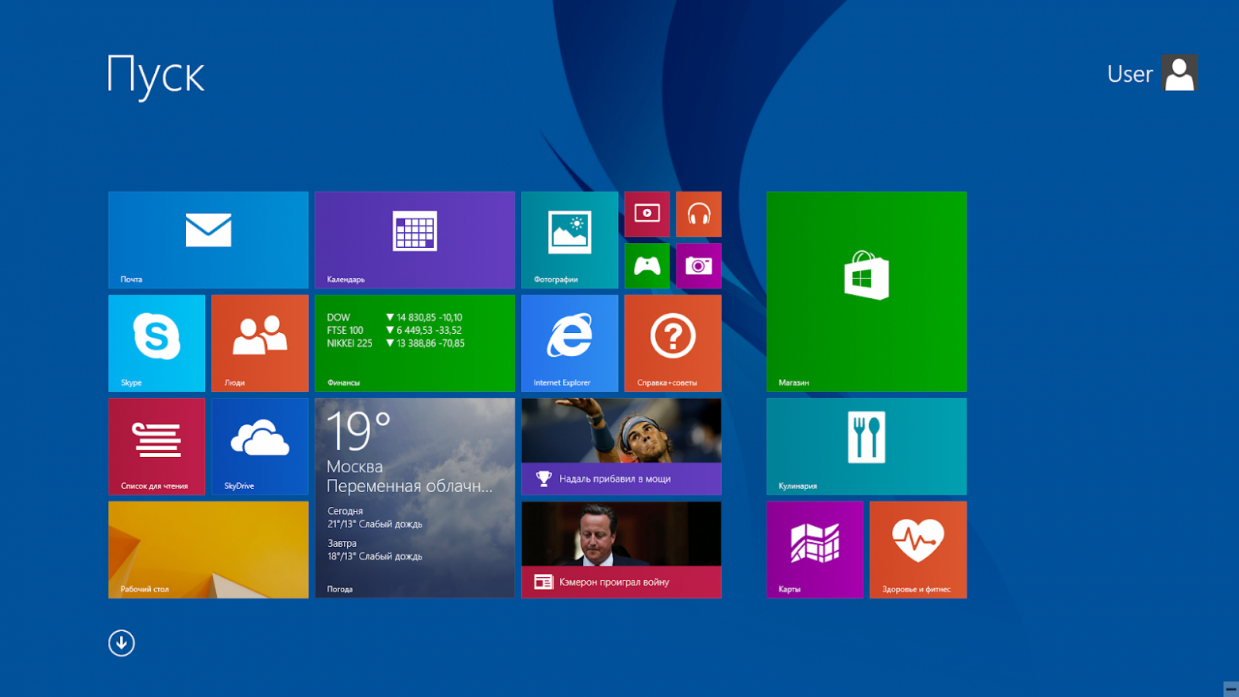
\includegraphics[width=1\textwidth]{imgs/11.1.png}}
    \textit{\caption{Windows 8.1}}
    \label{framework} %framework,fig1
\end{figure} \newpage


\begin{centering}
    \subsection*{Windows 10 — 30 сентября 2014 года}
\end{centering}

И вот, к 2015 году \textbf{Microsoft} выпускает \textbf{Windows 10}. При разработке \textbf{Microsoft} продолжала развитие идеи
единой системы для разных устройств. В «десятке» появилась голосовая помощница Кортана,
вернули меню «Пуск», улучшена системная безопасность. 

\begin{figure}[h]%current location
    \centering
    \scalebox{1}{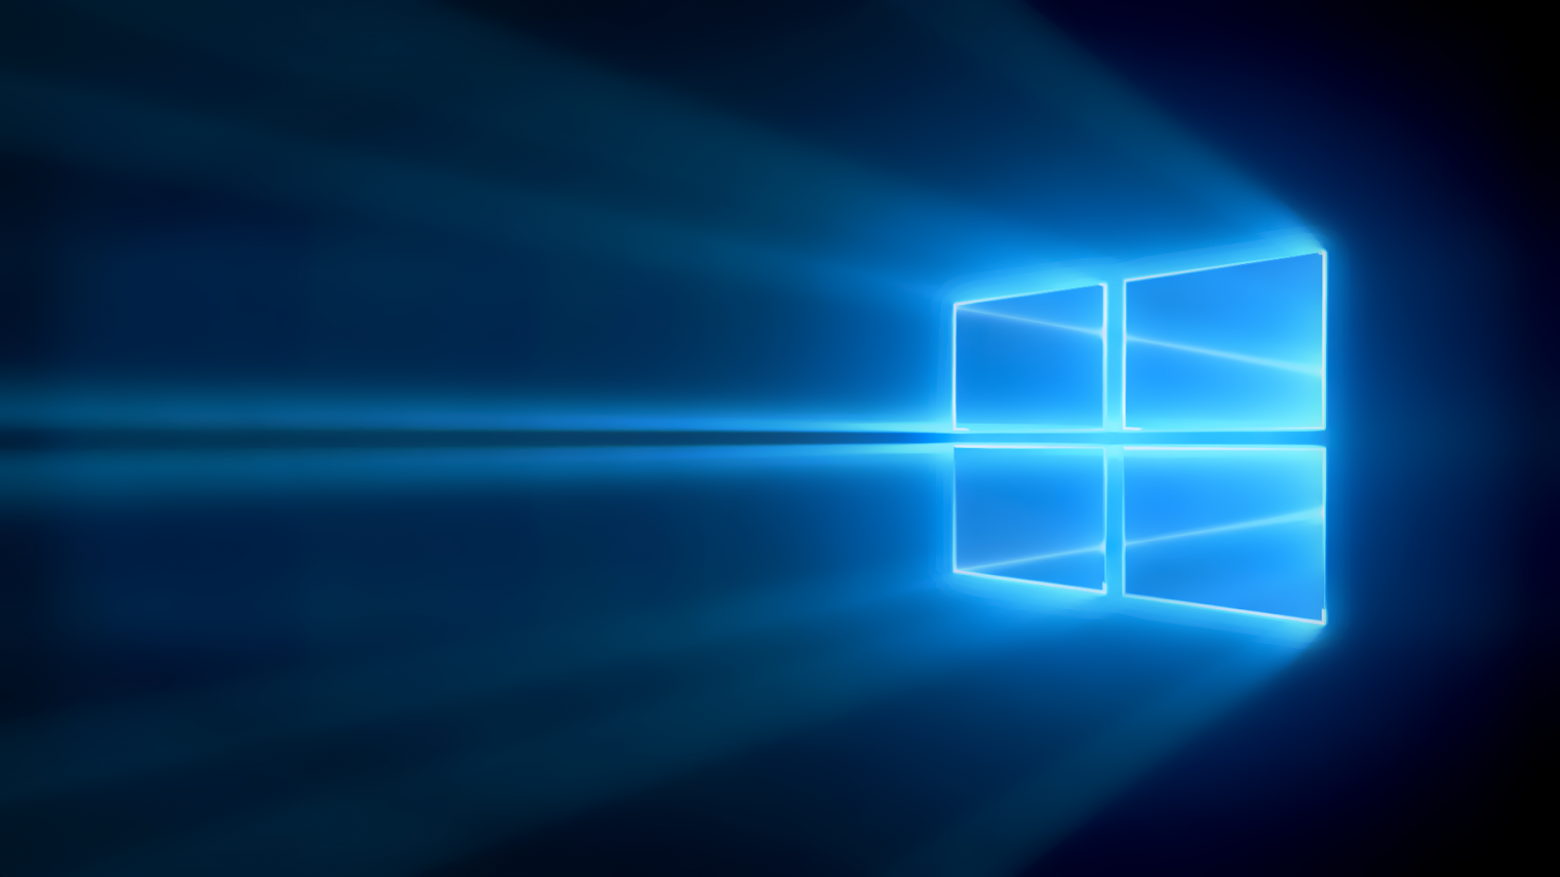
\includegraphics[width=1\textwidth]{imgs/12.1.png}}
    \label{framework} %framework,fig1
\end{figure} \newpage


\begin{centering}
    \subsection*{Windows 11 - 24 июня 2021 года}
\end{centering}

\begin{figure}[h]%current location
    \centering
    \scalebox{1}{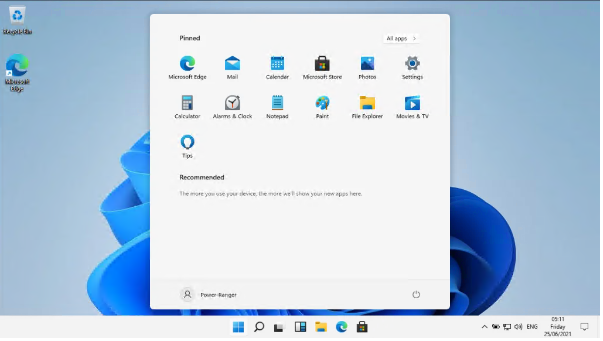
\includegraphics[width=1\textwidth]{imgs/13.1.png}}
    \label{framework} %framework,fig1
\end{figure}


\textbf{Windows 11} — операционная система для персональных компьютеров, разработанная в рамках семейства
\textbf{Windows NT}, чтобы стать преемницей \textbf{Windows 10}.

После шести лет существования \textbf{Windows 10}, самая популярная операционная система для компьютеров
получает крупное обновление до версии \textbf{Windows 11}. Хотя \textbf{Microsoft} заявляла,
что \textbf{Windows 10} будет последней версией этой ОС.


Правда, помимо интерфейса, важных изменений в \textbf{Microsoft Windows 11} немного. Да,
скруглённые углы окон, более стильными стали и диалоговые окна, но, большой доли ощущений,
как после перехода с \textbf{Windows 8} на \textbf{10}, на этот раз вы не испытаете. \newpage




\begin{center}
    \section*{Технические аспекты}
\end{center}

Чтобы осветить все технические аспекты и тонкости операционной системы \textbf{Windows} понадобится не менее
1000 страниц. Для особо любопытных советуем 7-е издание «\textbf{Внутреннего устройства Windows» Марка Руссиновича},
специалиста по внутреннему устройству Windows. Также можно почитать «Современные операционные системы»
Эндрю Таненбаума и «Operating System Concepts»: в обеих книгах есть главы, посвященные Windows.
Здесь же ограничимся рассмотрением инструментов взаимодействия приложений пользователя с операционной
системой (Windows API) и архитектуры «оси». \\


\begin{centering}
    \subsection*{Архитектура}
\end{centering}

Во многих многопользовательских операционных системах сама ОС отделяется от приложений.
Код ядра ОС выполняется в привилегированном режиме процессора (\textit{режим ядра}).
Для него доступны системные данные и оборудование. В непривилегированном режиме
(\textit{пользовательский режим}) выполняется код приложений. Ему предоставляется ограниченный набор
интерфейсов и ограниченный доступ к системным данным. Прямой доступ к оборудованию заблокирован.
При вызове программой пользовательского режима системной функции процессор выполняет специальную команду,
переключающую вызывающий поток (последовательность команд внутри процесса, планируемая \textbf{Windows} для исполнения)
в режим ядра. Когда системная функция завершается, операционная система переключает контекст
потока обратно в пользовательский режим и дает возможность вызывающей стороне продолжить работу.


\textbf{Windows} считается операционной системой с гибридным ядром. С одной стороны компоненты ядра \textbf{Windows}
располагаются в вытесняемой памяти и взаимодействуют друг с другом путем передачи сообщений,
как в микроядерных системах. С другой стороны ядро слишком велико (более 1 Мбайт), а большая
часть кода ОС и кода драйверов устройств использует одно защищенное пространство памяти
защищенного режима, что свойственно монолитным ОС. Это означает, что в теории любой компонент
ОС или драйвер устройства может повредить данные, используемые другими системными компонентами.
В \textbf{Windows} эта проблема решается за счет повышения качества и контроля происхождения сторонних
драйверов через такие программы, как \textbf{WHQL} или \textbf{KMCS}. Одновременно применяются дополнительные
технологии защиты ядра, такие как безопасность на базе виртуализации, функции \textbf{Device Guard}.

Рассмотрим ключевые системные компоненты, формирующие архитектуру системы.
На рисунке ниже представлена упрощенная схема, на которой опущены некоторые элементы,
например, сетевые компоненты и различные уровни драйверов. Первое, на что стоит обратить
внимание — это линия, разделяющая части пользовательского режима и режима ядра. Как упоминалось выше,
потоки пользовательского режима выполняются в закрытом адресном пространстве процессов.
На время выполнения в режиме ядра они получают доступ к системному пространству.
Таким образом, системные процессы, пользовательские процессы, процессы служб и подсистемы
среды обладают собственным закрытыми адресными пространствами.


\begin{figure}[h]%current location
    \centering
    \scalebox{1}{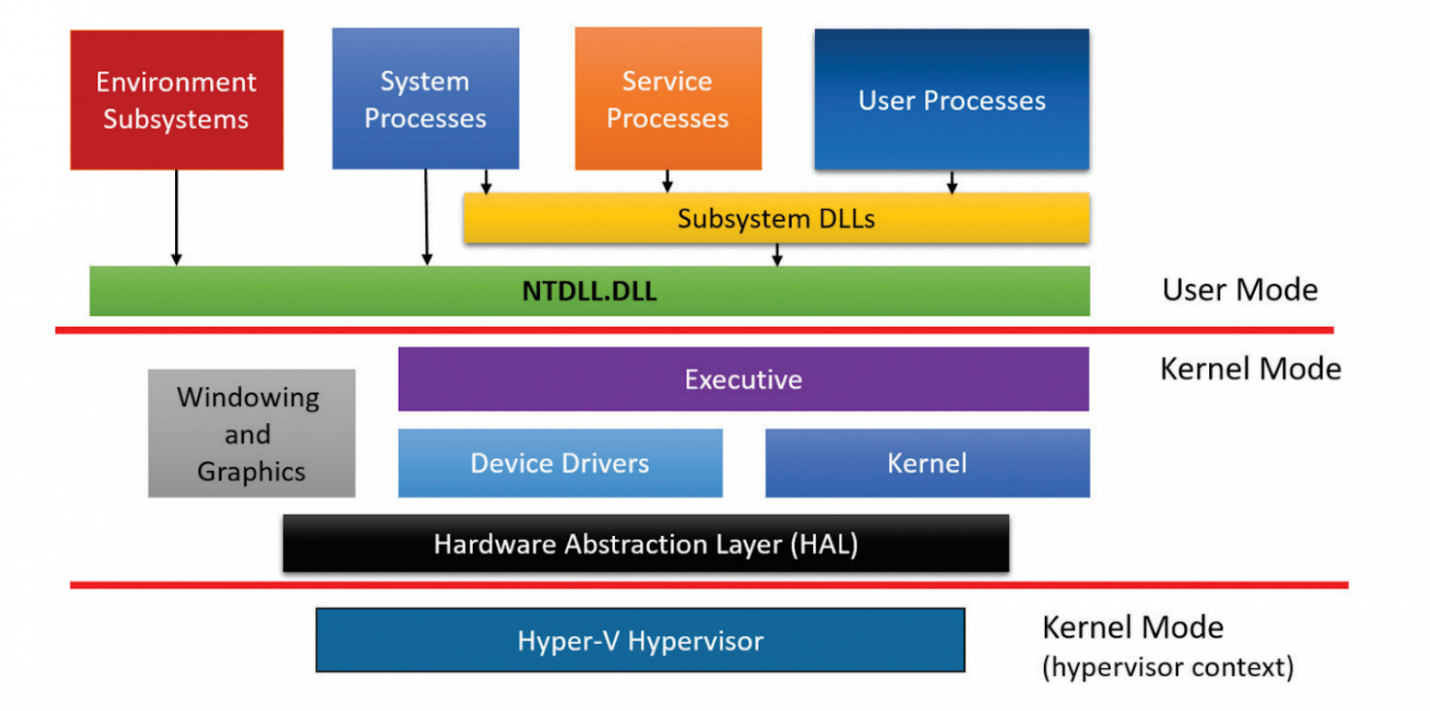
\includegraphics[width=1\textwidth]{imgs/14.1.png}}
    \textit{\caption{Упрощенная схема архитектуры Windows}}
    \label{framework} %framework,fig1
\end{figure} \newpage


Вторая линия разделяет компоненты режима ядра и гипервизор (Hyper-V). Гипервизор перехватывает
многие привилегированные операции, выполняемые ядром, и эмулирует их таким образом,
чтобы позволить на одной и той же машине одновременно работать нескольким операционными системам.
Гипервизор работает на том же уровне привилегий процессора (0), что и ядро. Но из-за
использования специализированных команд процессора (VT-x у процессоров Intel, SVM у АMD)
он может изолироваться от ядра с сохранением контроля над ним и приложениями.
Поэтому некоторые иногда применяют термин «кольцо -1». \\


Четыре базовых типа процессов пользовательского режима:
\begin{itemize}
    \item \textbf{Пользовательские процессы}. Эти процессы относятся к одному из следующих типов:
    32- или 64-разрядные приложения \textbf{Windows} (приложения \textbf{Windows Apps}, работающие на базе
    среды \textbf{Windows Runtime} в \textbf{Windows 8} и выше, включаются в эту категорию), 16-разрядные приложения \textbf{Windows 3.1},
    16-разрядные приложения b, 32- и 64-разрядные приложения \textbf{POSIX}. Заметим,
    что 16-разрядные приложения могут выполняться только в 32-разрядных версиях \textbf{Windows},
    а приложения \textbf{POSIX} в \textbf{Windows 8} уже не поддерживаются.

    \item \textbf{Процессы служб}. В эту категорию входят процессы, являющиеся хостами для
    служб \textbf{Windows} (например, службы планировщика задач и диспетчер печати).
    Обычно к службам предъявляется требование независимости выполнения от входа пользователя.
    Многие серверные приложения \textbf{Windows} (например, \textbf{Microsoft SQL Server} и \textbf{Microsoft Exchange Server})
    также включают компоненты, выполняемые как службы.

    \item \textbf{Системные процессы}. Фиксированные процессы, такие как процесс входа
    или диспетчер сеансов, не являются службами \textbf{Windows}. Другими словами,
    они не запускаются диспетчером служб.

    \item \textbf{Серверные процессы подсистем среды}. Такие процессы реализуют часть поддержки среды ОС,
    предоставляемой пользователю и программисту. Изначально в \textbf{Windows NT} было три подсистемы
    среды: \textbf{Windows}, \textbf{POSIX} и \textbf{OS/2}. Подсистема \textbf{OS/2} включалась только до \textbf{Windows 2000}, подсистема
    \textbf{POSIX} в последний раз была включена в \textbf{Windows XP}. \textbf{Ultimate-} и \textbf{Enterprise-} выпуски клиента
    \textbf{Windows 7}. Все серверные версии \textbf{Windows 2008 R2} включают поддержку расширенной подсистемы \textbf{POSIX},
    называемой \textbf{SUA} (\textbf{Subsystem for UNIX-based Applications}). Сейчас подсистема \textbf{SUA} не поддерживается
    и уже не включается как необязательное часть в версии \textbf{Windows} (\textbf{Windows 10} версии 1607 включает
    подсистему \textbf{Windows} для \textbf{Linux} — \textbf{WSL}, \textbf{Windows Subsystem for Linux}).
\end{itemize}


Обратим внимание на блок \textbf{DLL} подсистем под блоками Процессы служб и Пользовательские процессы.
В Windows пользовательские приложения не вызывают низкоуровневые сервисные функции операционной
системы напрямую. Вместо этого они проходят через одну или несколько \underline{динамических библиотек
(DLL)} подсистем. Их роль состоит в том, чтобы преобразовывать документированные функции в
соответствующие внутренние (недокументированные) вызовы системных функций, реализованных в
основном в Ntdll.dll. Преобразование может включать (а может не включать) отправку сообщения
процессу, обслуживающему пользовательский процесс.\\


Компоненты режима ядра:
\begin{itemize}
    \item \textbf{Исполнительная система}. Она содержит базовые сервисные функции
    ОС: управление памятью, управление процессами и потоками, безопасность,
    ввод/вывод, сетевая поддержка и межпроцессные коммуникации.

    \item \textbf{Ядро Windows}. Низкоуровневые функции ОС: планирование потоков,
    диспетчеризация прерываний и исключений и многопроцессорная синхронизация.
    Также ядро предоставляет набор функций и базовых объектов, которые используются
    исполнительной системой для реализации высокоуровневых конструкций.

    \item \textbf{Драйверы устройств}. Сюда входят как драйверы физических устройств,
    преобразующие вызовы пользовательских функций ввода/вывода в конкретные запросы
    ввода/вывода к устройству, так и драйверы устройств, не относящихся к
    физическому оборудованию, например драйверы файловой системы или сетевые драйверы.

    \item \textbf{Слой абстрагирования оборудования (\underline{HAL})}. Прослойка кода, изолирующее ядро,
    драйверы устройств и прочий исполняемый код Windows от платформенно-зависимых различий
    в работе оборудования, например различий между системными платами.

    \item \textbf{Оконная и графическая система}. Реализация функций графического интерфейса (GUI),
    также известных как функции GDI: работа с окнами, элементы пользовательского интерфейса и графический вывод.

    \item \textbf{Уровень гипервизора}. Включает всего-навсего один компонент:
    сам гипервизор. В этой среде нет ни драйверов, ни других модулей.
    При этом сам гипервизор состоит из нескольких внутренних уровней и служб:
    собственный диспетчер памяти, планировщик виртуальных процессов, управление
    прерываниями и таймером, функции синхронизации, разделы
    (экземпляры виртуальных машин) и внутрипроцессные коммуникации
    (IPC, Inter-Process Communication) и многие другие.
\end{itemize}


В таблице ниже представлены некоторые файлы некоторых базовых компонентов Windows:
\begin{center}
    \begin{tabularx}{\textwidth}{ |X|X| }
        \hline
        \begin{center}
            \textbf{Имя файла}
        \end{center}
         & 
        \begin{center}
            \textbf{Компоненты}
        \end{center} \\ [1.5ex]
          
        \hline
        Ntoskrnl.exe & Исполнительная система и ядро \\
        \hline   
        Hal.dll & HAL \\ 
        \hline
        Win32k.sys & Часть подсистемы Windows режима ядра (GUI) \\ 
        \hline
        Hvix64.exe (Intel), Hvax64.exe (AMD) & Гипервизор \\ 
        \hline
        .sys в $\backslash$SystemRoot$\backslash$System32$\backslash$Drivers & Основные файлы драйверов: DirectX, Volume Manager, TCP/IP и поддержка ACPI \\ 
        \hline
        Ntdll.dll & Внутренние вспомогательные функции и заглушки диспетчеризации системных сервисных функций \\
        \hline
        Kernel32.dll, Advapi32.dll, User32.dll, Gdi32.dll & Dll основных подсистем Windows \\
        \hline
    \end{tabularx}
\end{center}
    

\begin{centering}
    \subsection*{Windows API}
\end{centering}

\textbf{Windows API} (\textbf{Application Programming Interface}) — это программный интерфейс пользовательского режима для \textbf{Windows}.
До появления 64-разрядной версии операционной системы программный интерфейс 32-разрядных версий Windows
назывался Win32 API в отличие от исходного 16-разрядного Windows API (программный интерфейс для исходных
16-разрядных версий Windows). На данный момент термин Windows API или Win32 API относят как к 32-разрядным,
так и к 64-разрядным версиям.


В «доисторические времена» Windows API состоял только из функций в стиле C. Выбор языка Cбыл обусловлен тем,
что написанный на нем код также мог использоваться из других языков. Он являлся достаточно низкоуровневым
для предоставления сервиса ОС. Но огромное количество функций в сочетании с недостаточной последовательностью
выбора имен и отсутствием логических группировок (вроде пространств имен C++) привели к тому,
что в некоторых новых API используется другой механизм — модель COM.


\textbf{COM} базируется на двух основных принципах. Во-первых, клиенты взаимодействуют с объектами
(серверные объекты \textbf{COM}) через интерфейсы — четко определенные контракты с набором логически связанных методов,
сгруппированных посредством механизма диспетчеризации по виртуальным таблицам. Такой же механизм, к слову,
обычно применяется компиляторами C++ для реализации диспетчеризации виртуальных функций.
Таким образом обеспечивается двоичная совместимость и снимаются проблемы с декорированием имен компилятором.
Поэтому, такие методы могут вызываться из многих других языков и компиляторов, включая C, C++, VB, языки .NET,
Delphi и т. д. Вторым принципом является динамическая загрузка компонентов (вместо статической компоновки с клиентом).\\


\begin{centering}
    \subsection*{WinRT}
\end{centering}

В Windows 8 появился новый API и исполнительная среда поддержки Windows Runtime (WinRT).
WinRT состоит из платформенных сервисов, предназначенных для разработчиков приложений Windows Apps
(приложения Windows Apps подходят для устройств, начиная от миниатюрных IoT-устройств до телефонов,
планшетов, десктопных систем, ноутбуков и даже Xbox One и Microsoft HoloLens).


С точки зрения API платформа WinRT строится на базе COM, добавляя в базовую инфраструктуру
COM различные расширения. С архитектурной точки зрения она обладает намного большей целостностью:
в ней реализованы иерархии пространств имен, последовательная схема назначения имен и паттерны программирования.
На базовом двоичном уровне WinRT API все равно строится на основе унаследованных двоичных файлов и API Windows.
Это не новый «машинный» API для системы: ситуация немного напоминает то, как .NET строится на основе
традиционного Windows API.\\



\begin{centering}
    \subsection*{.NET Framework}
\end{centering}

.NET Framework является частью Windows. Он состоит из двух основных компонентов:
\begin{itemize}
    \item CLR (Common Language Runtime). Исполнительная среда .NET, включает JIT-компилятор
    для преобразования инструкций языка CIL в низкоуровневый язык машинных команд процессора,
    сборщик мусора, систему проверки типов, безопасность обращения к коду и т. д.
    Среда реализована в виде внутрипроцессного сервера COM (DLL) и использует различные средства,
    предоставляемые Windows API.
    \item .NET Framework Class Library (FCL). Обширная подборка типов, реализующих функциональность,
    часто используемую в клиентских и серверных приложениях, — средства пользовательского интерфейса,
    поддержка сети, работа с базами данных и т. д.
\end{itemize}


На схеме представлены отношения между .NET Framework и ОС Windows:
\begin{figure}[h]%current location
    \centering
    \scalebox{1}{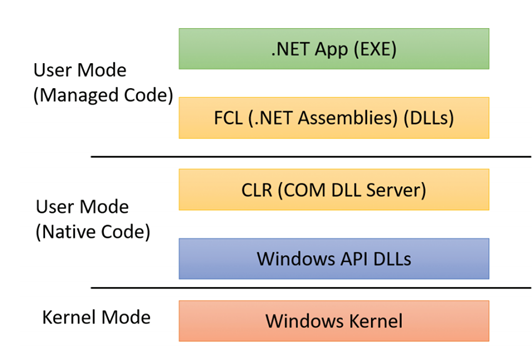
\includegraphics[width=1\textwidth]{imgs/15.1.png}}
    \label{framework} %framework,fig1
\end{figure} \newpage


\textit{Отношение между .NET и ОС Windows. Термин «сервер COM» обычно относится к DLL библиотеке или
исполняемому файлу (EXE), в котором реализованы классы COM.}
\end{document}
